\documentclass[ignorenonframetext,]{beamer}
\setbeamertemplate{caption}[numbered]
\setbeamertemplate{caption label separator}{: }
\setbeamercolor{caption name}{fg=normal text.fg}
\beamertemplatenavigationsymbolsempty
\usepackage{lmodern}
\usepackage{pifont}
\usepackage{amssymb}
\usepackage{booktabs}
%\usepackage{emoji}

\usepackage{hyperref}
\hypersetup{
    colorlinks=true,
    linkcolor=blue,
    filecolor=magenta,      
    urlcolor=cyan,
    pdftitle={Overleaf Example},
    pdfpagemode=FullScreen,
    }
    
\usepackage{color, colortbl}
\definecolor{LightCyan}{rgb}{0.88,1,1}
\usepackage{minted}
\usemintedstyle{borland}

\newcommand\Wider[2][3em]{%
\makebox[\linewidth][c]{%
  \begin{minipage}{\dimexpr\textwidth+#1\relax}
  \raggedright#2
  \end{minipage}%
  }%
}

\usepackage{amssymb,amsmath}
\usepackage{ifxetex,ifluatex}
\usepackage{fixltx2e} % provides \textsubscript
\ifnum 0\ifxetex 1\fi\ifluatex 1\fi=0 % if pdftex
  \usepackage[T1]{fontenc}
  \usepackage[utf8]{inputenc}
\else % if luatex or xelatex
  \ifxetex
    \usepackage{mathspec}
  \else
    \usepackage{fontspec}
  \fi
  \defaultfontfeatures{Ligatures=TeX,Scale=MatchLowercase}
\fi
% use upquote if available, for straight quotes in verbatim environments
\IfFileExists{upquote.sty}{\usepackage{upquote}}{}
% use microtype if available
\IfFileExists{microtype.sty}{%
\usepackage{microtype}
\UseMicrotypeSet[protrusion]{basicmath} % disable protrusion for tt fonts
}{}
\newif\ifbibliography
\hypersetup{
            pdftitle={Enrichissement de données de caisses à partir d’informations nutritionnelles : une approche par appariement flou sur données de grande dimension},
            pdfauthor={Lino Galiana},
            pdfborder={0 0 0},
            breaklinks=true}
\urlstyle{same}  % don't use monospace font for urls

% Prevent slide breaks in the middle of a paragraph:
\widowpenalties 1 10000
\raggedbottom

\AtBeginPart{
  \let\insertpartnumber\relax
  \let\partname\relax
  \frame{\partpage}
}
\AtBeginSection{
  \ifbibliography
  \else
    \let\insertsectionnumber\relax
    \let\sectionname\relax
    \frame{\sectionpage}
  \fi
}
\AtBeginSubsection{
  \let\insertsubsectionnumber\relax
  \let\subsectionname\relax
  \frame{\subsectionpage}
}

\setlength{\parindent}{0pt}
\setlength{\parskip}{6pt plus 2pt minus 1pt}
\setlength{\emergencystretch}{3em}  % prevent overfull lines
\providecommand{\tightlist}{%
  \setlength{\itemsep}{0pt}\setlength{\parskip}{0pt}}
\setcounter{secnumdepth}{0}
\setbeamertemplate{navigation symbols}{}
\setbeamertemplate{footline}[page number]

\title{Enrichissement de données de caisses à partir d’informations nutritionnelles}
\subtitle{Une approche par appariement flou sur données de grande dimension}
\author[shortname]{Lino Galiana\inst{1} ; Milena Suarez-Castillo\inst{2} ; Lionel Wilner\inst{1}}
\institute[shortinst]{\inst{1} D2E  \inst{2} SSP-lab}
\date{9 décembre 2021}

\begin{document}
\frame{\titlepage}

\begin{frame}
\tableofcontents[hideallsubsections]
\end{frame}

\section{Introduction}\label{sec: introduction}

\subsection{Démarche}
%lino

\begin{frame}{Objectif}{Problématique}

\begin{itemize}
    \item Alimentation affecte variables de santé publique ayant un effet de premier ordre sur bien-être :
\begin{itemize}
\item obésité
\item mortalité différentielle
\end{itemize}
\item Interaction avec les inégalités socioéconomiques: Caillavet et al. (2020)
\item Alcott et al. (2019) proposent une décomposition entre effets:
\begin{itemize}
\item d'offre (déserts alimentaires)
\item de demande (préférences pour la \textit{junk food})
\end{itemize}
\item Facteurs sociaux et territoriaux interagissent
\begin{itemize}
\item Malgré réglementations (ex: nutriscore), beaucoup d'asymétries d'information
\end{itemize}
\item Commencer par documenter les inégalités de "qualité" de consommation
\begin{itemize}
\item Avant d'essayer de distinguer effets offre et demande
\end{itemize}
\end{itemize}
    
\end{frame}

\begin{frame}{Objectif}{Problématique}

\begin{itemize}
    \item Au sein d'une classe de produit (ex: lasagnes), énormément d'hétérogénéité de "qualité"
\begin{itemize}
    \item Low-cost vs autres produits
    \item Bio vs agriculture traditionnelle
\end{itemize}
    \item Besoin de données très fines pour distinguer les qualités nutritionnelles (Caillavet et al. 2020)
    \item D'où l'utilisation de sources de collectes automatisées:
\begin{itemize}
    \item Données d'enquête (notamment Budget des Familles) serviront à vérifier la cohérence voire caler
    \item Autres sources administratives pour contrôler la qualité des données
\end{itemize}
\end{itemize}
\end{frame}

\begin{frame}{Objectif}{Enjeux}

\begin{itemize}
    \item Besoin d'enrichissements multiples:
\begin{itemize}
    \item Sur la dimension géographiques
    \item Sur la dimension produit
\end{itemize}
    \item Méthode des appariements flous 
\begin{itemize}
    \item Compenser absence d'identifiants pour appariements exacts
    \item Noms produits
    \item Adresse magasins
\end{itemize}
    \item Catégorisation pour réduire le nombre de paires
\begin{itemize}
    \item COICOP
    \item Département
\end{itemize}
\item Approche généralisable à de nombreux problèmes de la stat publique
\end{itemize}
\end{frame}


\subsection{Approche}
%milena

\section{Données}\label{sec: donnees}

\begin{frame}{RelevanC}

\begin{itemize}
    \item Données de caisses du groupe Casino
    \begin{itemize}
        \item Casino, Monoprix, Franprix au niveau magasin et 
        \item Leader Price et des petites chaînes (stations services, Sherpa...) au niveau magasin exclusivement
    \end{itemize}
    \item $\approx$ 11 000 magasins
    \item $\approx$ 250 000 produits
\end{itemize}

\end{frame}

\begin{frame}{RelevanC}
\makebox[\textwidth]{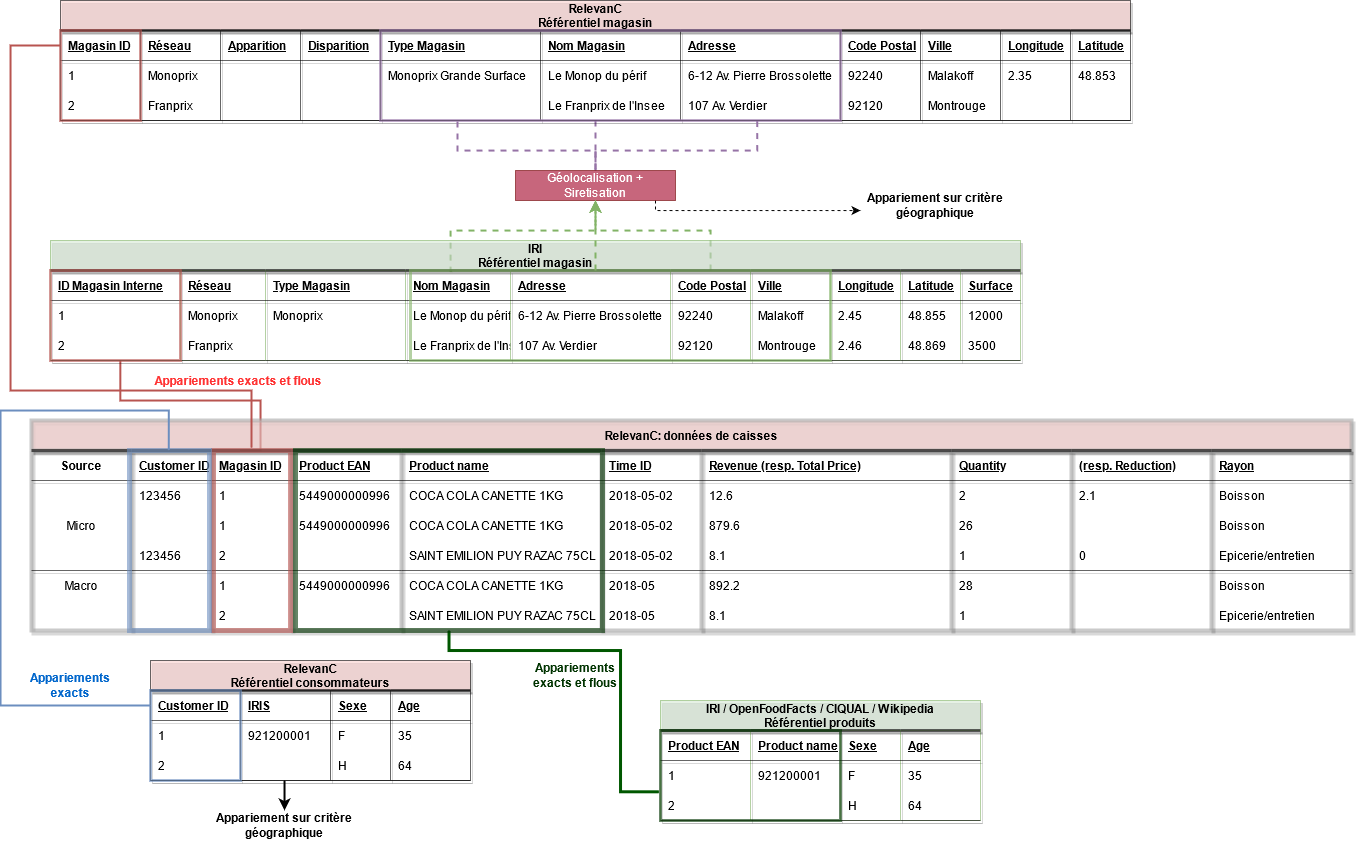
\includegraphics[width=\paperwidth]{images/schema-structure.drawio.png}}
\end{frame}

\begin{frame}{OpenFoodFacts}{\href{https://fr.openfoodfacts.org}{openfoodfacts.org}}

\begin{itemize}
    \item Base de données contributive et open-source (alternative à \texttt{Yuka})
\begin{itemize}
    \item Actualisée en continu
    \item Mise à disposition de csv de manière quotidienne
    \item Plusieurs API
\end{itemize}
    \item $\approx$ 2 millions de produits
    \item Beaucoup d'infos disponibles
\begin{itemize}
    \item Scores de qualité agrégés : nutriscore, score NOVA, écoscore
    \item Infos nutritionnelles: calories, glucides, lipides, etc.
    \item Infos sur produit: packaging, etc.
\end{itemize}
    \item \textit{Challenge}:  qualité et taux de complétude variable
\begin{itemize}
    \item Valeurs manquantes
    \item Erreurs de remplissage et fautes d'ortographe
\end{itemize}
\end{itemize}
\end{frame}

\begin{frame}{CIQUAL}{\href{https://ciqual.anses.fr/}{ciqual.anses.fr}}

\begin{itemize}
    \item Base de données élaborée par l'Anses
    \item Produits standardisées
    \item Beaucoup d'infos disponibles
    \item \textit{Challenge}:  meilleure qualité mais produits standardisés
\begin{itemize}
    \item Perte d'une dimension dans l'hétérogénéité produit
    \item Globalement même information qu'\texttt{OpenFoodFacts}
\end{itemize}
    \item Besoin d'enrichir certaines classes de produits:
\begin{itemize}
    \item Faible variabilité nutritionnelle
    \item Forte hétérogénéité des labels des sous-classes: marques, domaines, goûts...
\end{itemize}
    
\end{itemize}
\end{frame}
\begin{frame}{Dictionnaires de produits via Wikipédia}{\href{https://www.mediawiki.org/wiki/API}{https://www.mediawiki.org/wiki/API}}
    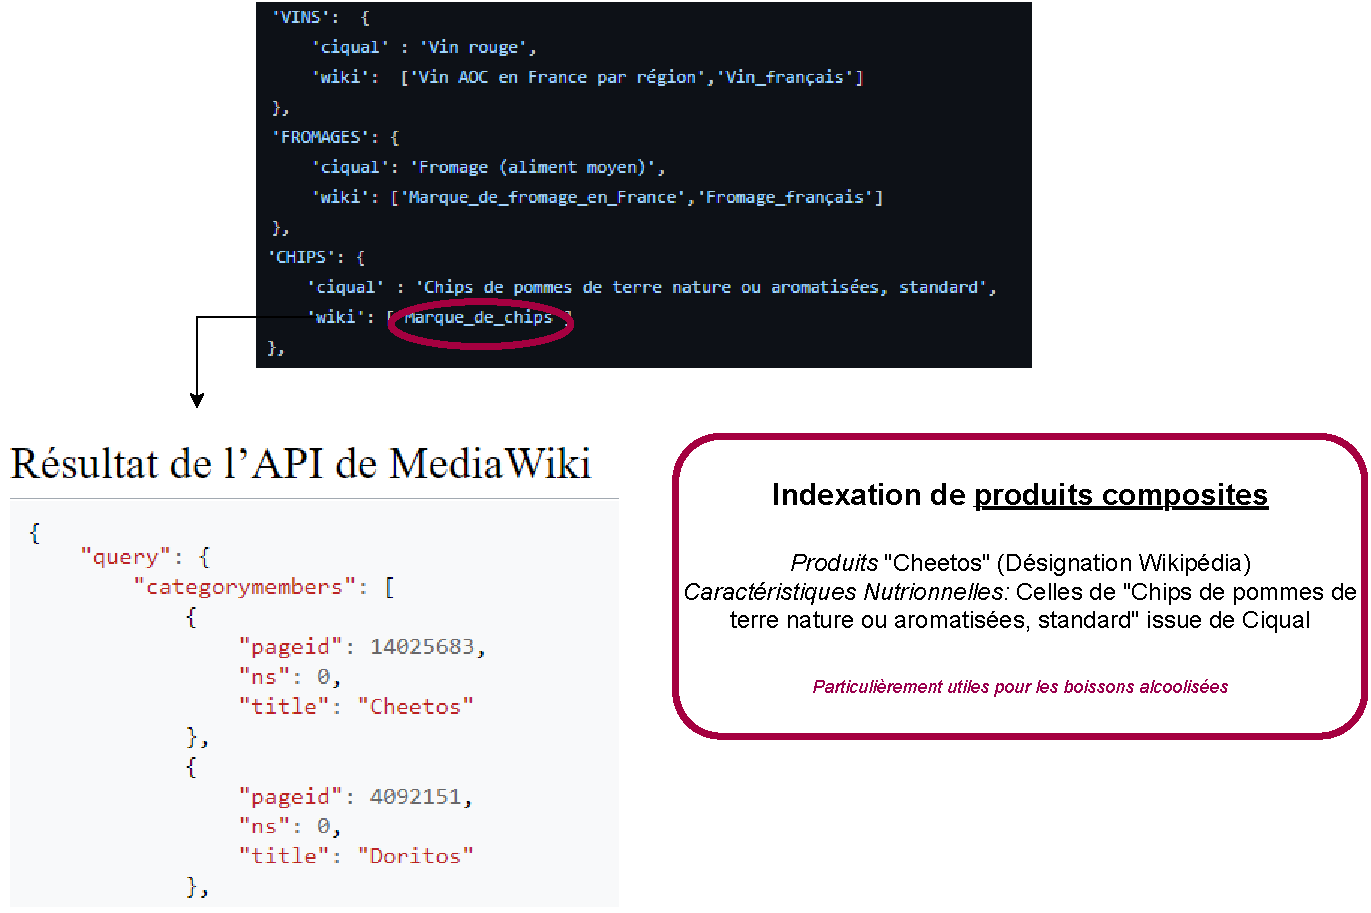
\includegraphics[width = \linewidth]{images/wikipedia.pdf}
    
\end{frame}

\begin{frame}{Modèle Fasttext \texttt{COICOP}}

Réutilisation d'un output du projet \texttt{PAul-EAN}: modèle de prédiction de la classe COICOP entrainé sur \textit{l'ensemble} des données de caisse à deux niveaux:

\begin{itemize}
    \item COICOP prédite comme variable de blocage
    \item Création d'une \textit{distance} ad-hoc entre libellés via un plongement de mots, qui est initialisé sur le plongement de mots issu de ce modèle 
\end{itemize}
    
\end{frame}

\section{Appariement produit}\label{sec: appariement produit}

\subsection{Vue globale}

\begin{frame}{Schéma macro du pipeline}

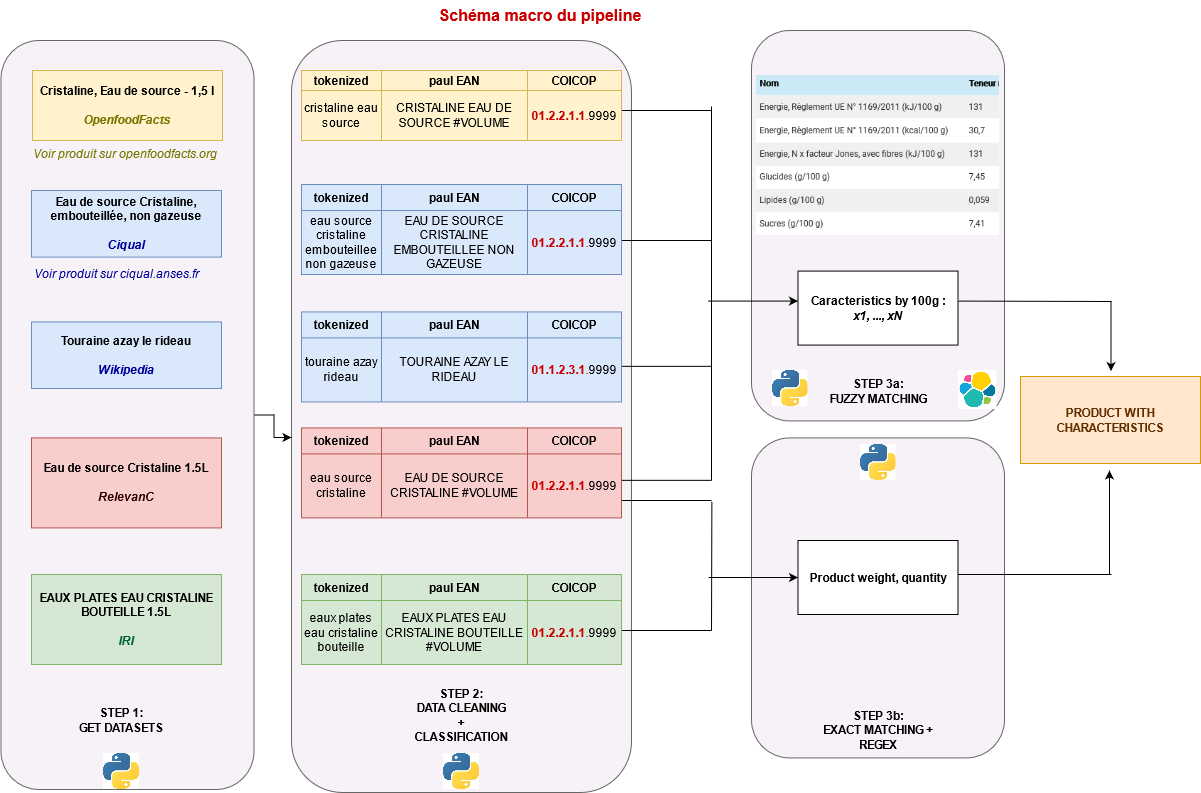
\includegraphics[width = \linewidth]{images/macro.png}

\end{frame}

\subsection{Data cleaning et catégorisation}

\begin{frame}{Data cleaning et catégorisation}
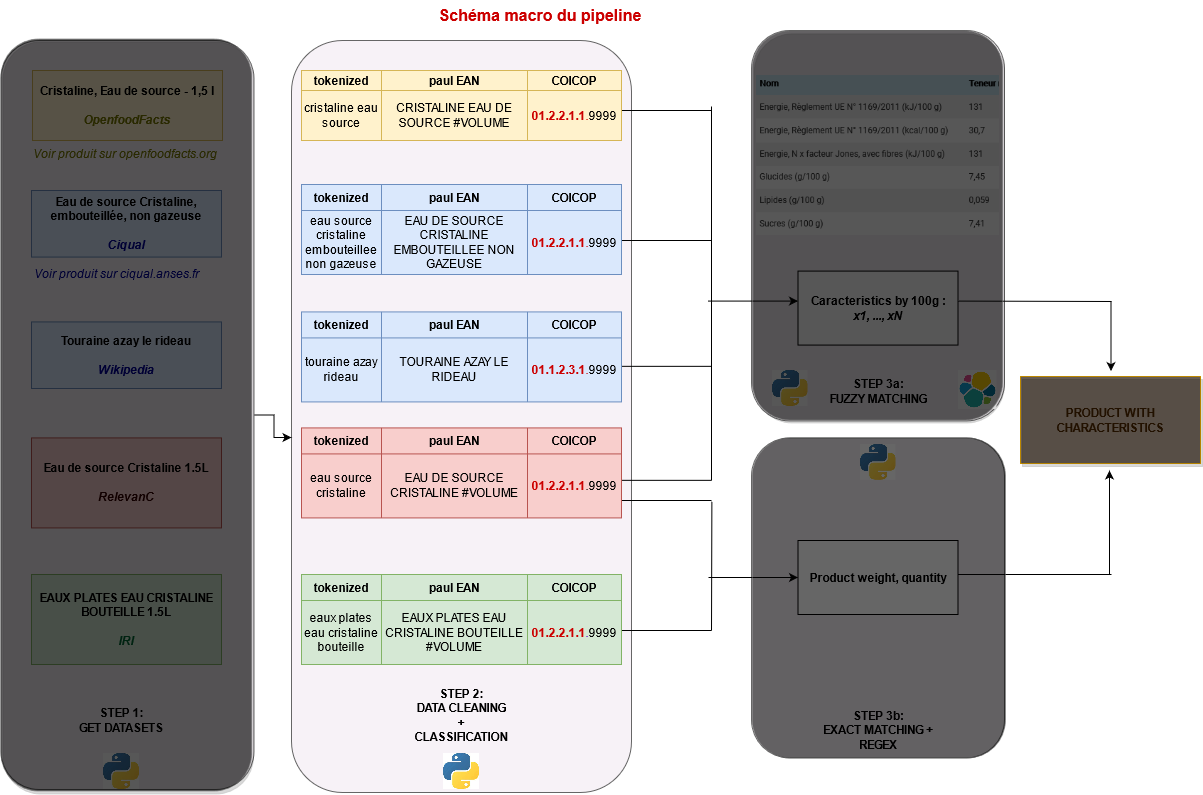
\includegraphics[width = \linewidth]{images/macro-ombre2.png}
\end{frame}

\begin{frame}{Enjeu du data cleaning}

\begin{itemize}
    \item Réduire le bruit dans les données ;
    \item Harmoniser les jeux de données ;
    \item Détecter des produits non alimentaires malgré filtre rayons.
\end{itemize}

    \begin{figure}[ht]
        \begin{minipage}[b]{0.45\linewidth}
            \centering
            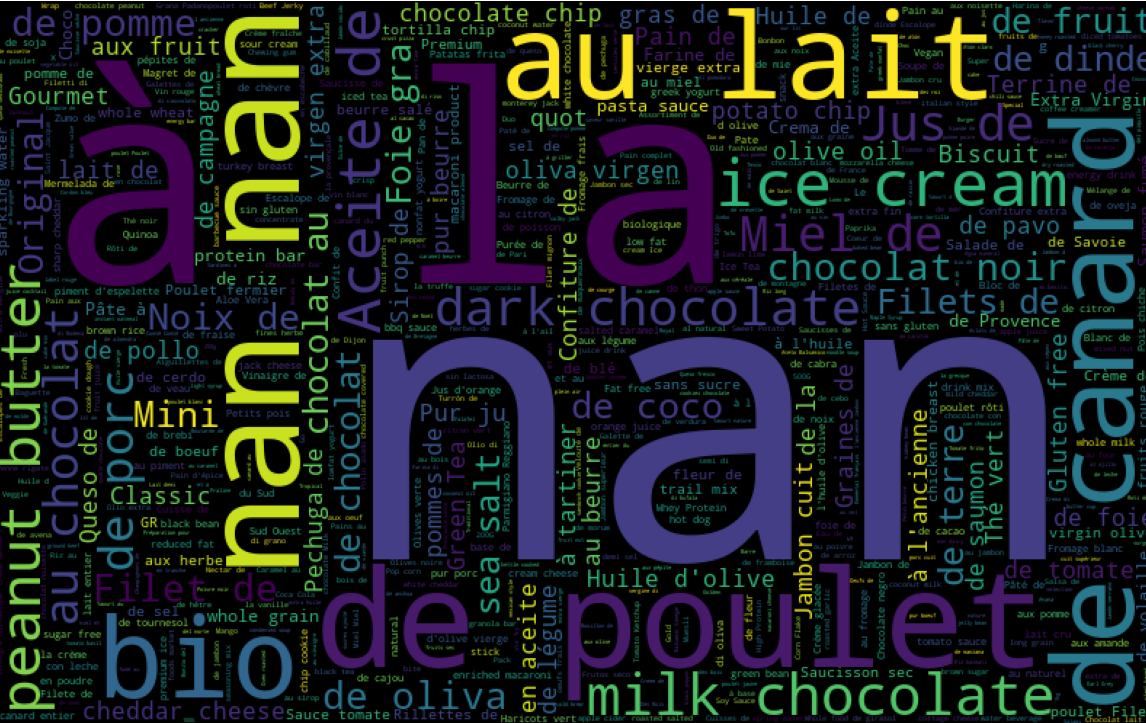
\includegraphics[width=\textwidth]{images/openfood_start.png}
            \caption{OpenfoodFacts}
            \label{fig: wordcloud openfood}
        \end{minipage}
        \hspace{0.5cm}
        \begin{minipage}[b]{0.45\linewidth}
            \centering
            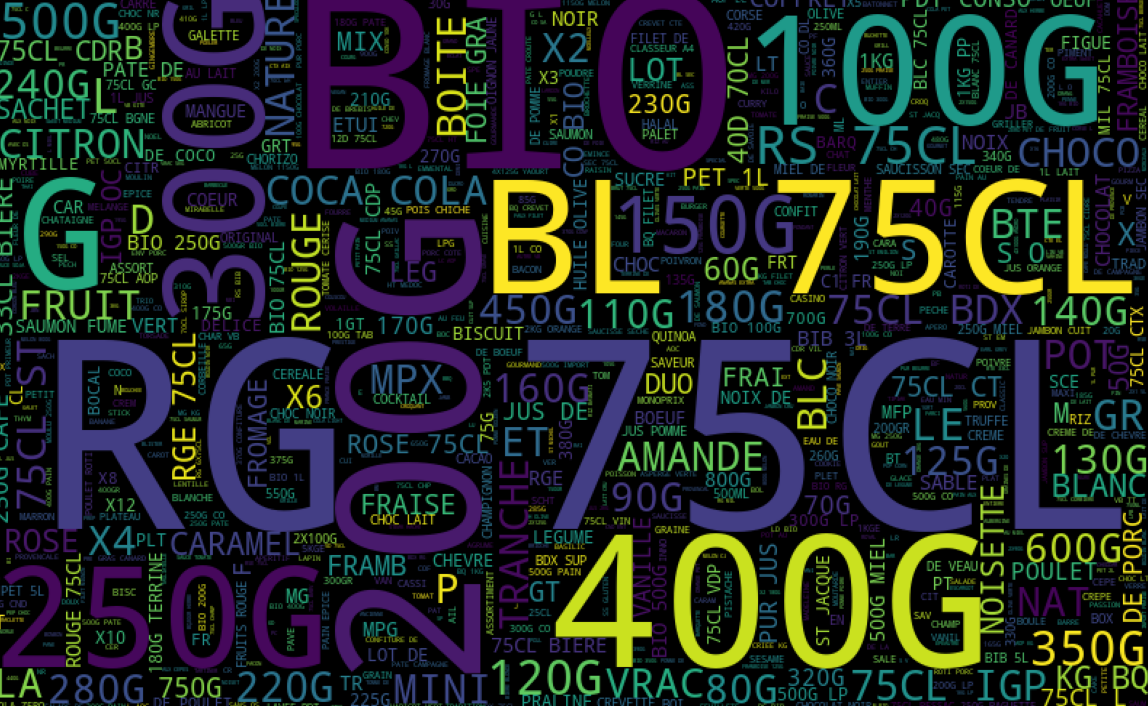
\includegraphics[width=\textwidth]{images/relevanc_start.png}
            \caption{RelevanC}
            \label{fig: wordcloud relevanc}
        \end{minipage}
        \caption{Nuages de mots avant pre-processing}
    \end{figure}


\end{frame}
    
\end{frame}

\begin{frame}{Pipeline de data-cleaning}

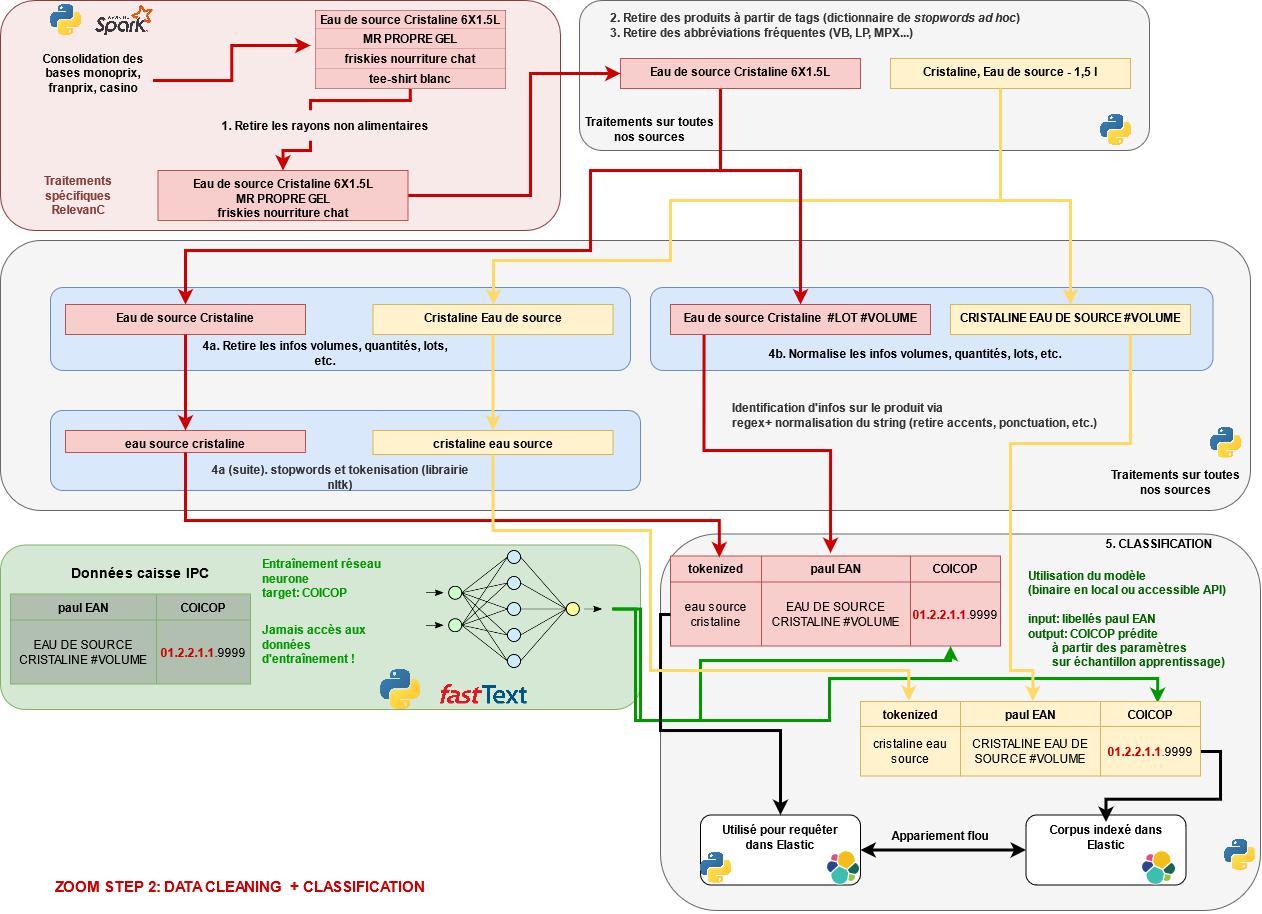
\includegraphics[width = \linewidth]{images/step2-cleaning-categorisation.drawio.png}

\end{frame}


\begin{frame}{Pipeline de data-cleaning}{Premières étapes: définir le champ le plus précis et cohérent possible}

\begin{enumerate}
    \item Consolidation des bases des différentes chaînes
    \item Elimine des produits non alimentaires (\texttt{RelevanC} et \texttt{OpenFood})
    \item Retire des abbréviations qui apportent du bruit
\end{enumerate}

\begin{center}
\makebox[\textwidth]{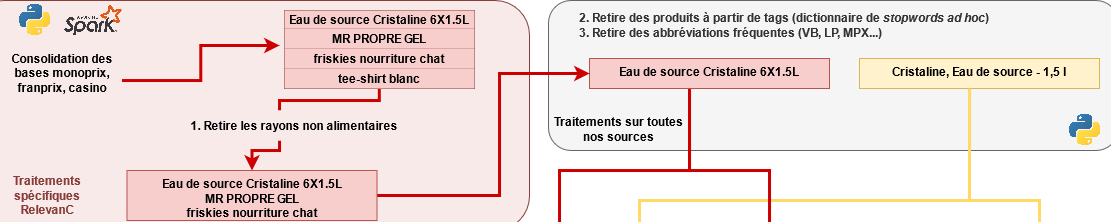
\includegraphics[width=\paperwidth]{images/step2-cleaning-categorisation-part1.png}}
\end{center}

\end{frame}

\begin{frame}{Pipeline de data-cleaning}{Deuxième étape: normalisation des noms de produits}

\begin{enumerate}
\setcounter{enumi}{3}
    \item Identification par expression régulière d'infos sur le produit
\begin{itemize}
    \item Remplacement par des mots-clés (\texttt{\#VOLUME}, \texttt{\#POIDS}, \texttt{\#UNITE}, \texttt{\#LOT}...) pour la classification
    \item Suppression de ces infos pour le libellé d'appariement flou
\end{itemize}    
\end{enumerate}

Un exemple: 

\begin{footnotesize}
\inputminted{python}{example-regex.py}
\end{footnotesize}

\begin{center}
\makebox[\textwidth]{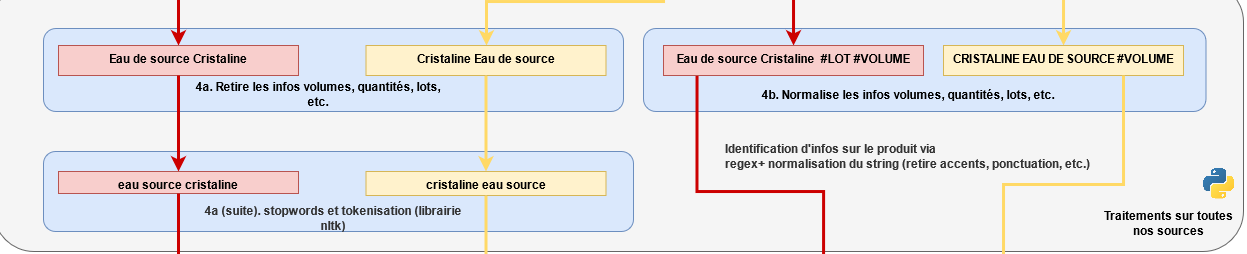
\includegraphics[width=\paperwidth]{images/step2-cleaning-categorisation-part2.png}}
\end{center}

\end{frame}

\begin{frame}{Pipeline de data-cleaning}{Deuxième étape: normalisation des noms de produits}

\begin{enumerate}
\setcounter{enumi}{4}
\item Transformation en suite d'unités signifiantes (\textit{token})
\begin{itemize}
    \item Retrait des \textit{stopwords} qui n'apporte pas d'info sur le produit 
    \item Mots comme token
    \item \texttt{nltk} plutôt que \texttt{spaCy}
    \item Pas de \textit{stemming}
    \item Les n-grams sont définis au niveau de la requête \texttt{Elastic}
\end{itemize}
\end{enumerate}

\begin{center}
\makebox[\textwidth]{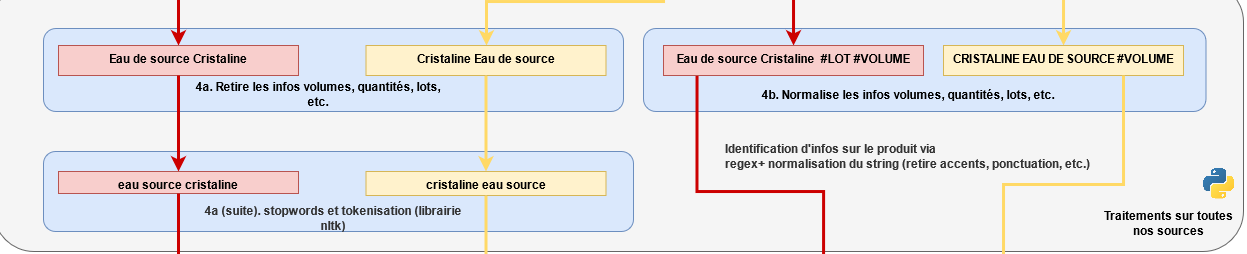
\includegraphics[width=\paperwidth]{images/step2-cleaning-categorisation-part2.png}}
\end{center}

\end{frame}

\begin{frame}{Pipeline de data-cleaning}{Deuxième étape: normalisation des noms de produits}

\begin{itemize}
    \item[\rlap{\raisebox{0.3ex}{\hspace{0.4ex}\scriptsize \ding{52}}}$\square$] Réduire le bruit dans les données ;
    \item[\rlap{\raisebox{0.3ex}{\hspace{0.4ex}\scriptsize \ding{52}}}$\square$] Harmoniser les jeux de données ;
    \item[\rlap{\raisebox{0.3ex}{\hspace{0.4ex}\scriptsize \ding{52}}}$\square$] Détecter des produits non alimentaires malgré filtre rayons.
\end{itemize}

    \begin{figure}[ht]
        \begin{minipage}[b]{0.45\linewidth}
            \centering
            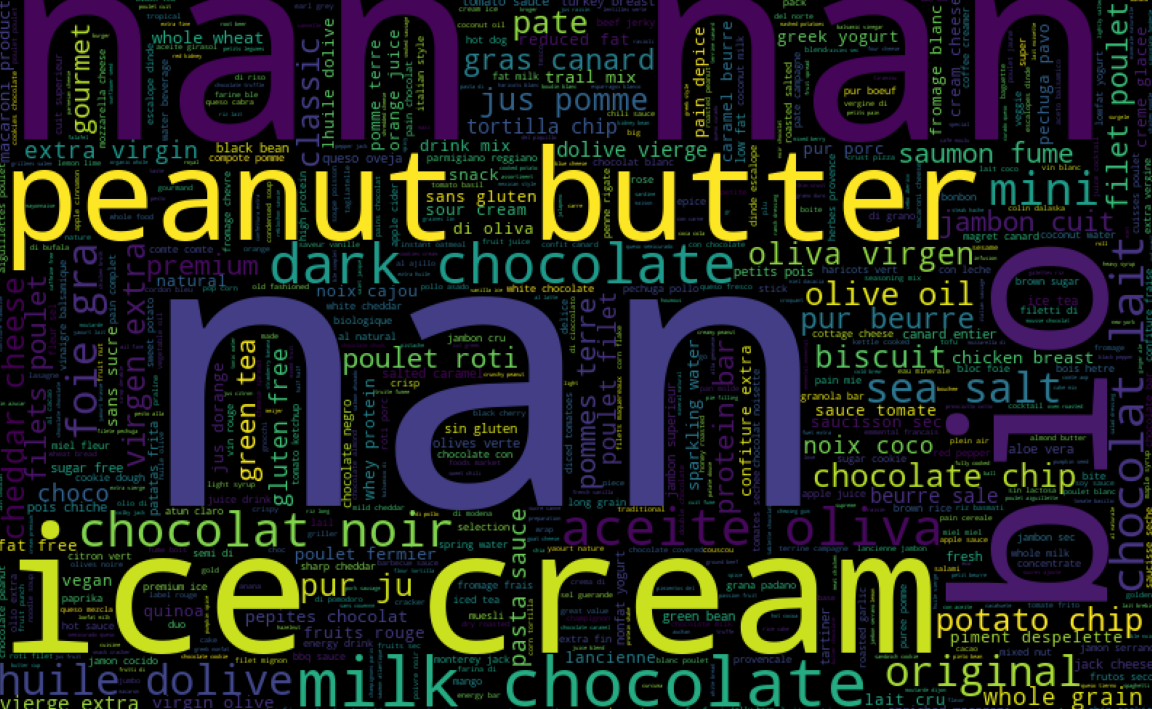
\includegraphics[width=\textwidth]{images/openfood_tokenized.png}
            \caption{OpenfoodFacts}
            \label{fig: wordcloud openfood}
        \end{minipage}
        \hspace{0.5cm}
        \begin{minipage}[b]{0.45\linewidth}
            \centering
            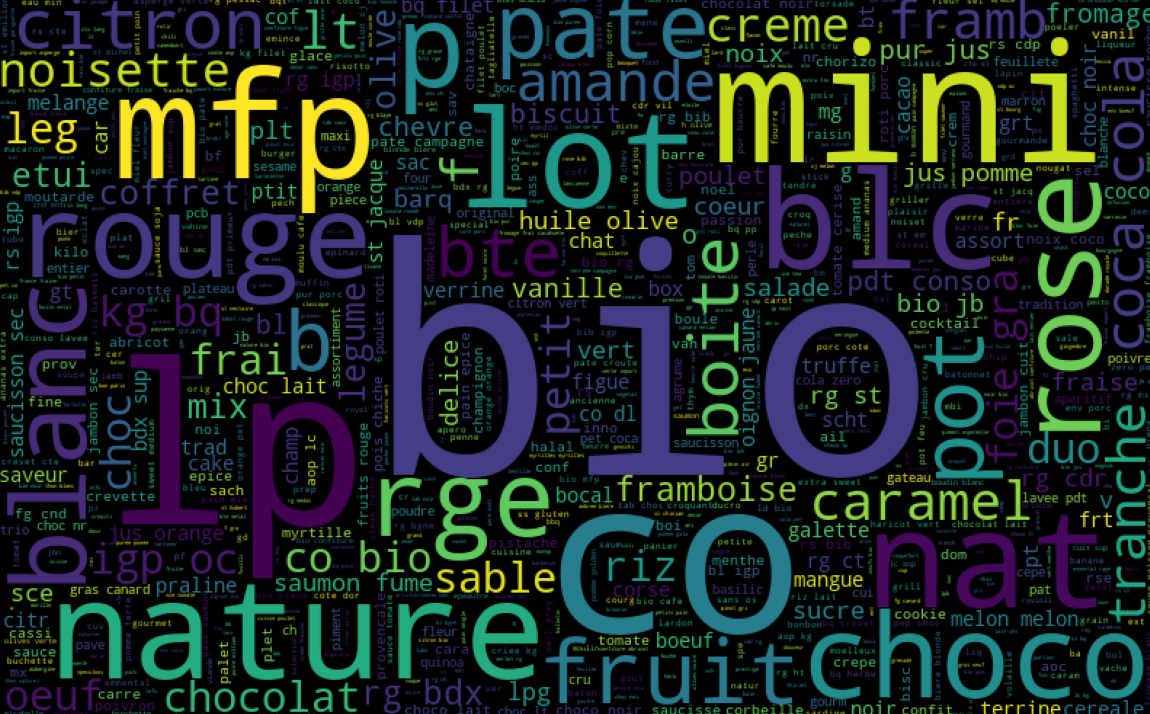
\includegraphics[width=\textwidth]{images/relevanc_tokenized.png}
            \caption{RelevanC}
            \label{fig: wordcloud relevanc}
        \end{minipage}
        \caption{Nuages de mots avant pre-processing}
    \end{figure}


\end{frame}

\begin{frame}{Pipeline de data-cleaning}{Deuxième étape: normalisation des noms de produits}

\Wider{
\begin{footnotesize}
\begin{tabular}{p{0.35\linewidth}p{0.25\linewidth}p{0.35\linewidth}}
\toprule
                \multicolumn{1}{c}{\textbf{Libellé d'origine}} & \multicolumn{1}{c}{\textbf{Libellé tokenisé}}        &          \multicolumn{1}{c}{\textbf{Libellé classification}}               \\
\midrule
\rowcolor{LightCyan}
                  NUTELLA POT 225G &                nutella pot &                 NUTELLA POT \#POIDS  \\
          PULCO DELICE AGRUME 70CL &        pulco delice agrume &        PULCO DELICE AGRUME \#VOLUME  \\
\rowcolor{LightCyan}
Cristaline Eau de source - 1,5 l &      cristaline eau source &   CRISTALINE EAU DE SOURCE \#VOLUME  \\
             COCA COLA CANETTE 1KG &          coca cola canette &           COCA COLA CANETTE \#POIDS  \\
           Brioche tranchée nature &    brioche tranchee nature &             BRIOCHE TRANCHEE NATURE \\
\rowcolor{LightCyan}
               °RELIGIEUSE CAFE X2 &         degreligieuse cafe &            DEGRELIGIEUSE CAFE \#LOT  \\
1/2 CHEVREAU S/TET S/ABA 2,5KG ENV &       chevreau tet aba env &    12 CHEVREAU STET SABA \#POIDS ENV \\
\rowcolor{LightCyan}
   SAINT EMILION PUY RAZAC RG 75CL & saint emilion puy razac & SAINT EMILION PUY RAZAC RG \#VOLUME  \\
\bottomrule
\end{tabular}
\end{footnotesize}
}

\end{frame}

\begin{frame}{Classification}{Classement dans la COICOP}

\begin{itemize}
    \item Chercher un nom de produit proche dans $\approx$ 2 millions est une tâche excessivement complexe...
    \item ... surtout quand on doit le faire 250 000 fois
    \item Equivalent à un produit cartésien de $10^{13}$ opérations (nombre de cellules dans le corps humain)
    \item Trouver une variable de blocage pour n'associer qu'une partie des paires entre-elles:
    \begin{itemize}
        \item Améliore la pertinence de la recherche
        \item Réduit drastiquement la complexité du problème
    \end{itemize}
    \item Pas de variable commune dans nos différentes sources:
    \begin{itemize}
        \item Rayon: faible qualité, pas correspondance 
    \end{itemize}
    \item Utilisation COICOP
\end{itemize}
    
\end{frame}

\begin{frame}{Classification}{Classement dans la COICOP}

\begin{itemize}
    \item Réseau neurone entraîné sur données de caisses
    \item Utilisation des poids estimés grâce au binaire \texttt{fasttext}
    \item Jamais accès aux données d'entraînement
    \item Classement à un niveau très fin (plus fin que niveau poste)
    \begin{itemize}
        \item \texttt{01.2.2.1.1}: \textit{Eaux minérales et de source}
    \end{itemize}
\end{itemize}

\begin{center}
\makebox[\textwidth]{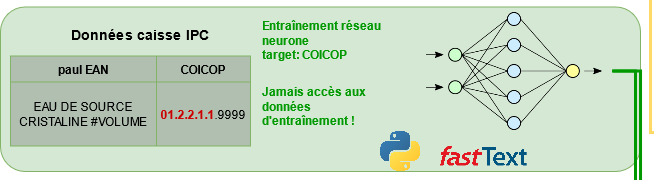
\includegraphics[width=\paperwidth]{images/step2-cleaning-categorisation-part3.png}}
\end{center}
    
\end{frame}

\begin{frame}{Classification}{Exemples}

\begin{footnotesize}
\begin{tabular}{p{0.35\linewidth}p{0.25\linewidth}p{0.35\linewidth}}
\toprule
                \multicolumn{1}{c}{\textbf{Libellé d'origine}} & \multicolumn{1}{c}{\textbf{Libellé tokenisé}}        &          \multicolumn{1}{c}{\textbf{Libellé classification}} \\
\midrule
                  NUTELLA POT 225G &     01.1.8.3.2.0001 &               Confiseries à base de chocolat \\
\rowcolor{LightCyan}
          PULCO DELICE AGRUME 70CL &     01.2.2.2.1.9999 &                    Boissons rafraîchissantes \\
             COCA COLA CANETTE 1KG &     01.2.2.2.1.0005 &                    Boissons rafraîchissantes \\
\rowcolor{LightCyan}
  Cristaline Eau de source - 1,5 l &     01.2.2.1.1.9999 &                  Eaux minérales ou de source \\
              CITRONS VERTS FILETS &     01.1.9.4.1.0006 &                        Plats cuisinés n.c.a. \\
\rowcolor{LightCyan}
           Brioche tranchée nature &     01.1.1.3.1.0001 &                                         Pain \\
               °RELIGIEUSE CAFE X2 &     05.6.1.2.1.9999 & Petits articles pour l'entretien du logement \\
\rowcolor{LightCyan}
1/2 CHEVREAU S/TET S/ABA 2,5KG ENV &     01.1.2.3.1.9999 &                     Mouton, agneau et chèvre \\
   SAINT EMILION PUY RAZAC RG 75CL &     02.1.2.1.2.0005 &                              Vins supérieurs \\
\bottomrule
\end{tabular}
\end{footnotesize}


\end{frame}


\subsection{Enrichissement des données de caisse}

\begin{frame}{Appariement}{Pipeline général}

\begin{itemize}
    \item On recherche dans OpenFood/CIQUAL un produit des données de caisses
    \item Une procédure pour aller de l'appariement le plus certain
au plus incertain
\begin{enumerate}
    \item Appariement EAN si disponible dans OpenFood
    \item Appariement flou dans les produits OpenFood ayant le même code COICOP
    \item Appariement flou dans tous les produits OpenFood
    \item Appariement flou dans tous les produits CIQUAL (enrichie avec le dico Wikipedia)
\end{enumerate}
\item Critères de validation conservateurs pour exclure faux positifs
\end{itemize}

\end{frame}

\subsection{Enrichissement des données de caisse}

\begin{frame}{Appariement}{Pipeline général}

\begin{itemize}
    \item Code \texttt{Python} pour gérer ce \textit{pipeline}
    \item Package \texttt{foodbowl} %\emoji{ramen} %{\fontspec{Symbola}\symbol{"1F35C}}
\begin{enumerate}
    \item Gère la connexion à S3 et Elastic
    \item Mise en forme des requêtes, récupération des échos...
    \item Validation des \textit{outputs} (distance textuelle et potentiellement réseau de neurone \texttt{PyTorch})
    \item Déploiement sous forme d'API grâce à \texttt{fastAPI} (à venir)
\end{enumerate}
\end{itemize}

\end{frame}

\begin{frame}{Etape 1}{Appariement EAN}

\begin{itemize}
    \item EAN est un identifiant produit unique (en principe...)
    \item Permet un appariement exact entre \texttt{RelevanC} et \texttt{OpenFood}
    \item Pour la calorie (catégorie la mieux renseignée): permet d'enrichir 46\% des données \texttt{RelevanC}
\end{itemize}
\end{frame}



\begin{frame}{Etape 2}{Objectif du fuzzy matching}

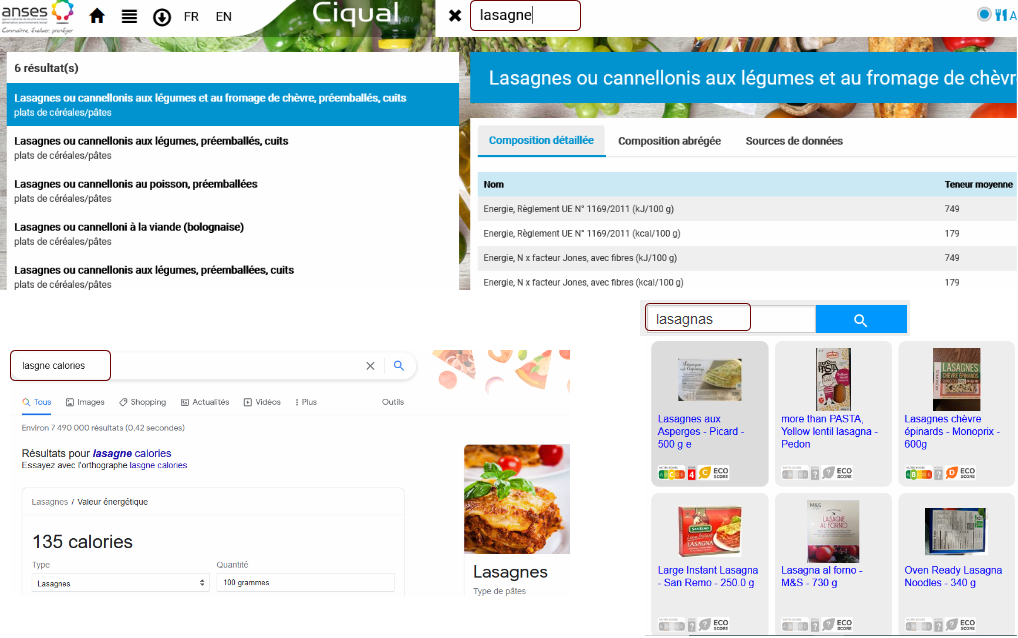
\includegraphics[width = \linewidth]{images/elastic-openfood-lasagnas.drawio.png}

\end{frame}

\begin{frame}{ElasticSearch}

\begin{tabular}{lr}
\toprule
{Implémentation} &  Nombre de secondes \\
\midrule
elastic    &            0.92 \\
rapidfuzz  &           97.20 \\
fuzzywuzzy &           99.90 \\
\bottomrule
\end{tabular}
    
\end{frame}

\begin{frame}{Critère de validation}
\begin{itemize}
    \item \texttt{rapidfuzz.fuzz.partial\_ratio(s\_1, s\_2)}: meilleure similarité entre la chaîne de caractère la plus courte \texttt{s\_1}, de longueur \texttt{n} et les \texttt{n}-grammes de  \texttt{s\_2}
    \item Similarité : distance de Levenshtein (y compris transposition) normalisée par la longueur $n$
    \item \texttt{partial\_ratio(s\_1, s\_2) > 0.65}
    
\end{itemize}
   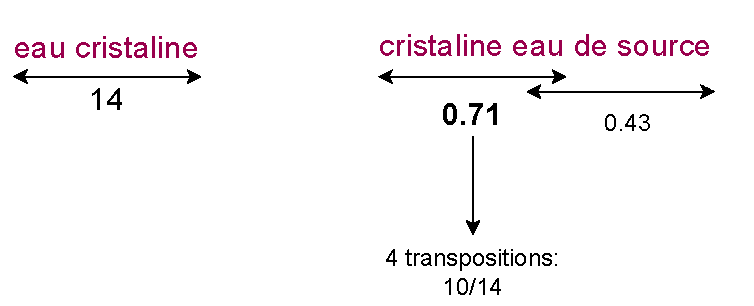
\includegraphics[width=0.8\linewidth]{images/partial_ratio.pdf}
    
\end{frame}

\begin{frame}{Une distance adaptée à notre problème?}
La proximité de caractère n'implique pas nécessairement une proximité sémantique.

\begin{footnotesize}
\begin{tabular}{p{0.35\linewidth}p{0.35\linewidth}}
\toprule
                \multicolumn{1}{c}{\textbf{Libellé d'origine}} & \multicolumn{1}{c}{\textbf{Libellé du match}}     
\midrule
                  oe poulet blanc fermier &    poulet blanc fermier 	 \\
\rowcolor{LightCyan}
          tarte chevre epinar co 	 & epinar \\
            lapin or sous alu 	 & oeufs sous alu 	 \\
\bottomrule
\end{tabular}
\end{footnotesize}

\begin{itemize}
    \item Test d'un plongement de mots: associer à un libellé un vecteur dans $\mathbb{R}^N$
    \item En déduire une distance non exclusivement basée sur la chaîne de charactère
\end{itemize}

\end{frame}
\begin{frame}{}
    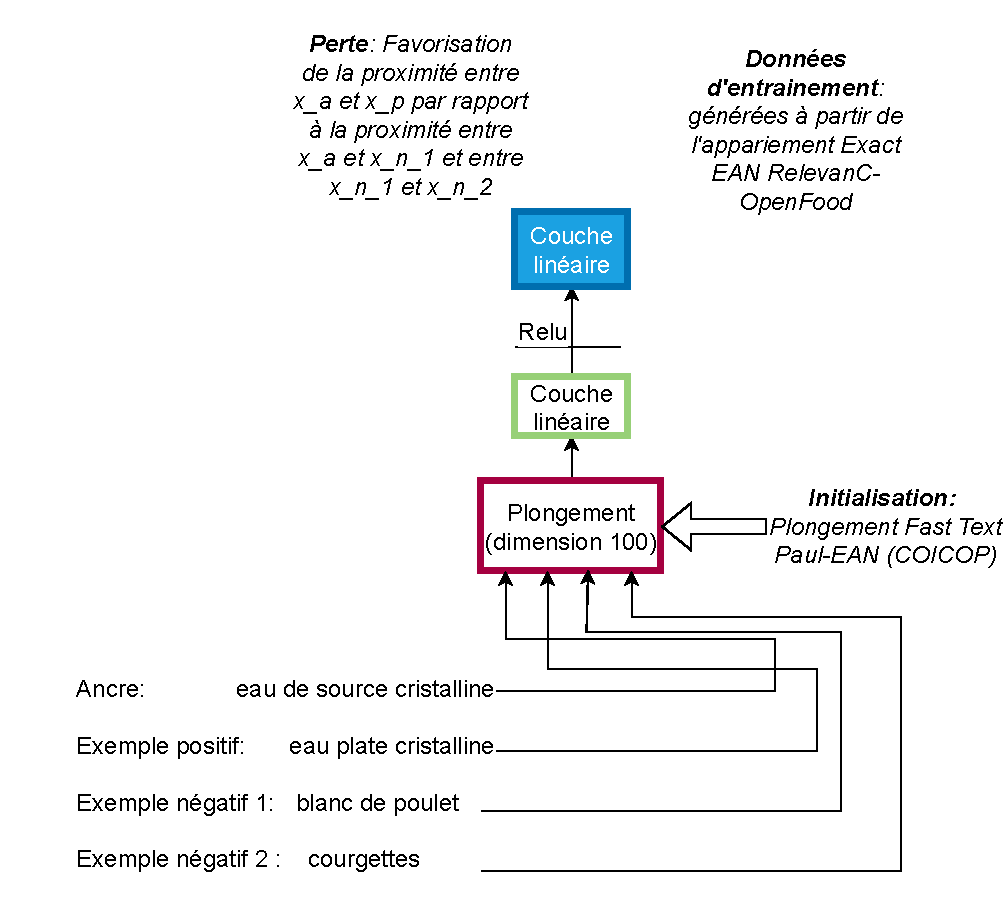
\includegraphics[width=\linewidth]{images/siamese.pdf}
\end{frame}
\begin{frame}{Bilan}
    \begin{itemize}
    \item Appariement alternatif: indexer les vecteurs "libellés OpenFood", et aller chercher le plus proche voisin de chaque vecteur "libellé relevanC"
        \item Sur l'appariement avec OpenFood: des performances qui semblent similaires à la pipeline présentée jusqu'ici
        \item Coûteux à intégrer à la pipeline: à ce stade pas envisagé puisque les résultats obtenus semblent déjà satisfaisant
        \item Utile cependant pour repérer les faux positifs/produire un score de confiance par comparaison des résultats des deux méthodes
    \end{itemize}
\end{frame}
\section{Appariement magasin}\label{sec: appariement magasin}

\begin{frame}{Schéma Macro}
    \makebox[\textwidth]{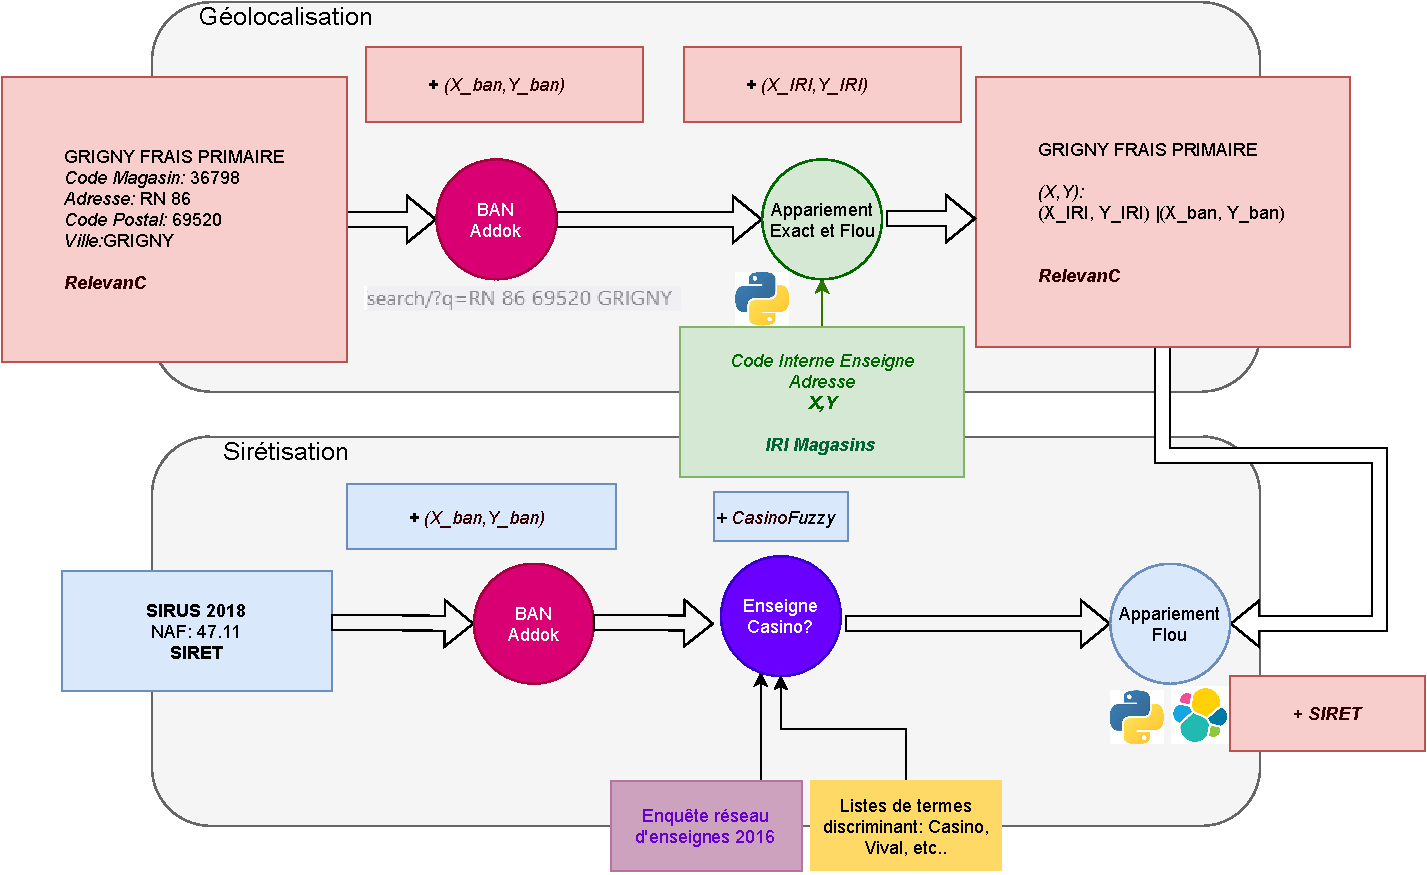
\includegraphics[width=0.98\paperwidth]{images/macro_localim.pdf}}
\end{frame}
\begin{frame}{}
        \makebox[\textwidth]{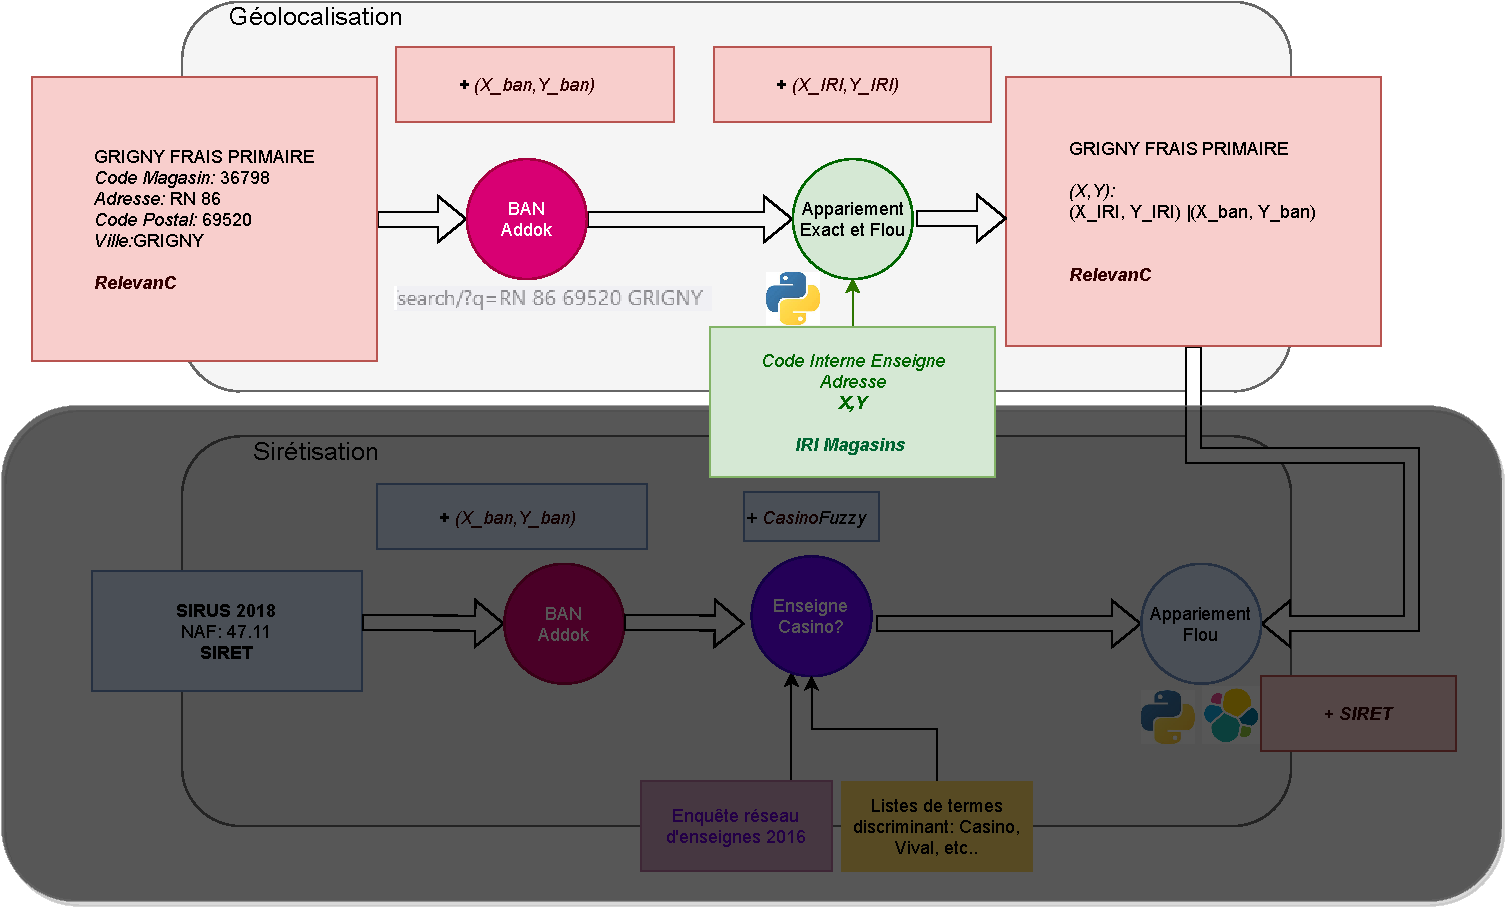
\includegraphics[width=0.98\paperwidth]{images/macro_geoloc.pdf}}
\end{frame}
\begin{frame}{Géolocalisation à partir de la BAN}
        \makebox[\textwidth]{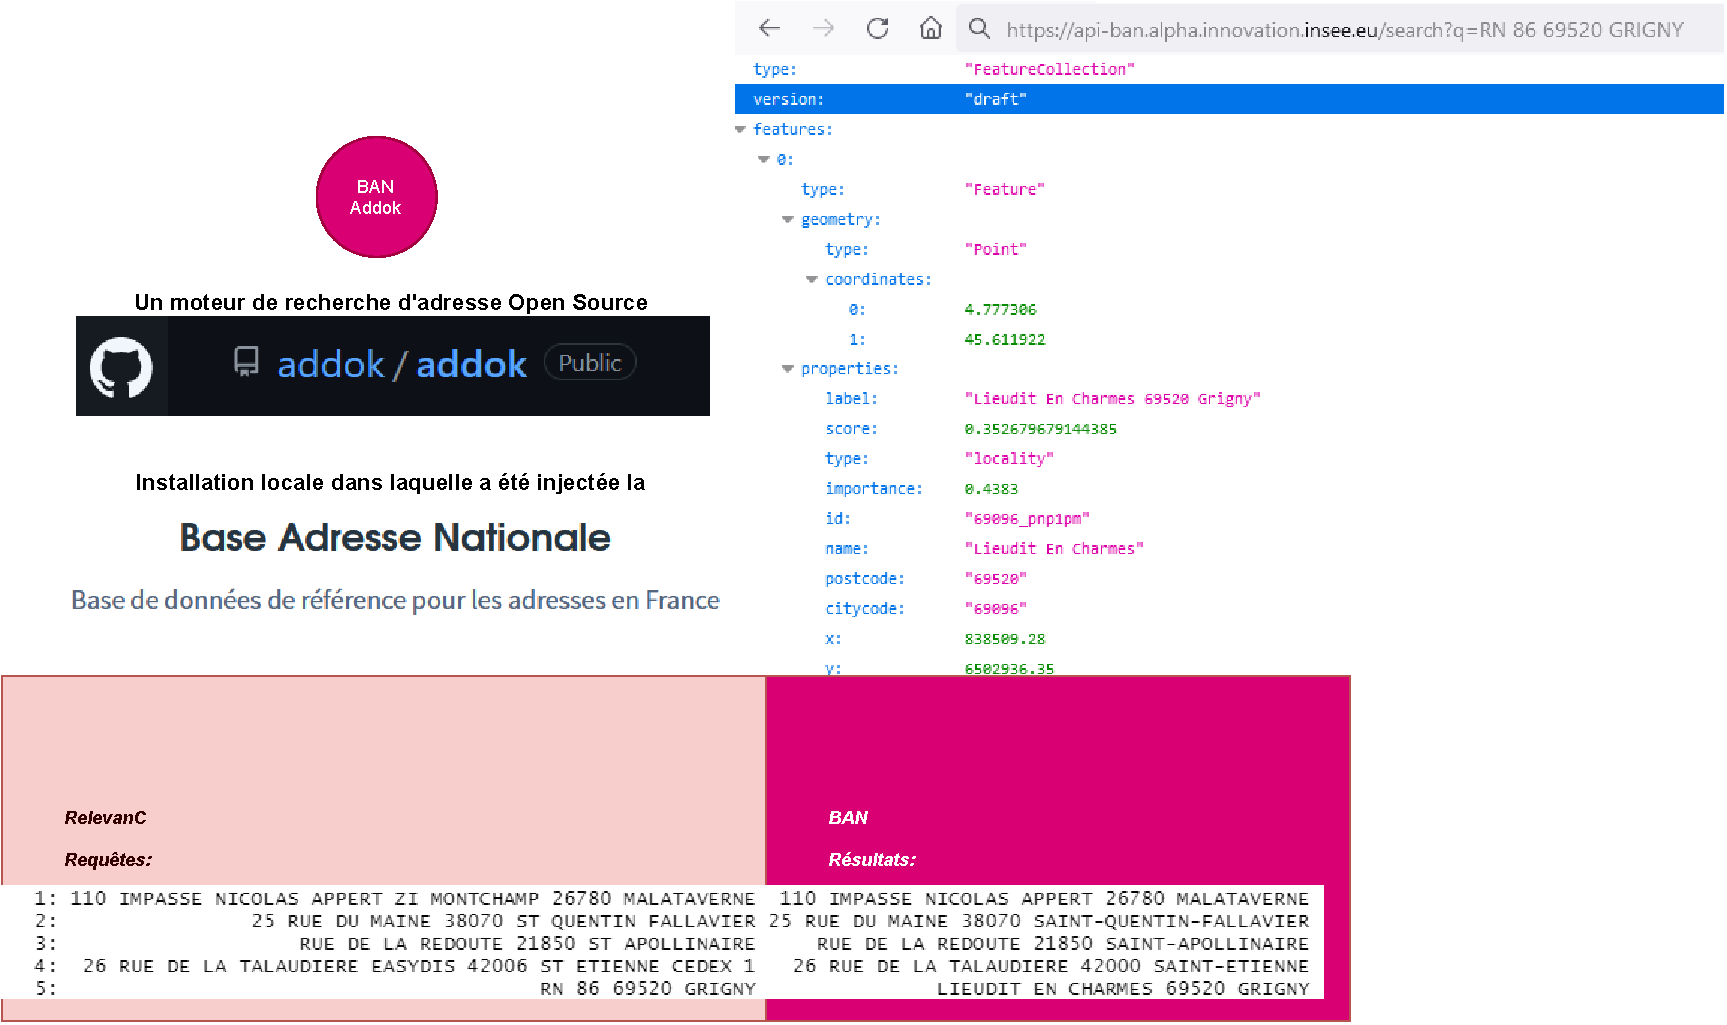
\includegraphics[width=0.98\paperwidth]{images/addok.pdf}}
\end{frame}
\begin{frame}{Géolocalisation par rapprochement à IRI}
\begin{enumerate}
    \item Appariement Exact: à partir d'un code interne magasin (par enseigne) disponible dans le répertoire IRI
    \item Appariement Flou: à l'aide de la librarie python \textit{recordLinkages}
\end{enumerate}

Recherche d'un match à partir de 
\begin{itemize}
    \item \textit{Blocage:} Code Postal; \textit{Champ comparé et noté:} Nom du magasin, Libellé d'enseigne, Adresse \textit{(string)} et X,Y \textit{(Point géographique)}. 
    $$m_1 > 3 $$ 
    \item \textit{Blocage:} Département; \textit{Champ comparé et noté:} Nom du magasin, Libellé d'enseigne, Adresse, Ville \textit{(string)} et X,Y \textit{(Point géographique)}
    $$m_2 > 5 $$ 
\end{itemize}

\tiny{
    $m_1 = 3 \times SimLev(Adresse)\times (SimLev(Adresse)>0.6) + 2  \times SimLev(Enseigne) \times (SimLev(Enseigne)>0.9) + \\ 
    1.5  \times SimGeo(X,Y) + 0.5  \times SimLev(Denom)\times(SimLev(Denom)>0.2) $ 
    
    \
    
    $m_2 = 3 \times SimLev(Ville)\times (SimLev(Ville)>0.8) + 2 \times SimLev(Adresse)\times (SimLev(Adresse)>0.6) + 1  \times SimLev(Enseigne) \times (SimLev(Enseigne)>0.9) + \\ 
    1  \times SimGeo(X,Y) + 1  \times SimLev(Denom)\times(SimLev(Denom)>0.2) $}
\end{frame}

\begin{frame}{Géolocalisation}{Bilan}

\begin{footnotesize}
\begin{tabular}{p{0.2\linewidth}c{0.1\linewidth}c{0.1\linewidth}c{0.1\linewidth}}
\toprule
                 &  & \multicolumn{2}{c}{\textbf{dont:}} \\
                \multicolumn{1}{c}{\textbf{Origine X,Y}} & \multicolumn{1}{c}{\textbf{Magasins}}        &          \multicolumn{1}{c}{\textbf{Autre X,Y}} &          \multicolumn{1}{c}{\textbf{Au moins 1 désaccord (>1km)}} \\
\midrule
                 Relevanc  & 470           &      464 &  31\\
\rowcolor{LightCyan}
          IRI: Exact &  3516   &   3465 & 412  \\
           IRI: Flou&  3428      &         3419 &  329 \\
           \rowcolor{LightCyan}
Addok-BAN &  4089         &          0  &   0 & \\
NA & 113              &     0  &  0 \\
\bottomrule
\end{tabular}


\end{footnotesize}

\

Parmi les magasins géolocalisé en "IRI exact" et en "Addok-Ban", distance entre les deux options (m):

\

\begin{footnotesize}
\begin{tabular}{c{0.1\linewidth}c{0.1\linewidth}c{0.1\linewidth}c{0.1\linewidth}}
\toprule
                \multicolumn{1}{c}{\textbf{10\%}} & \multicolumn{1}{c}{\textbf{50\%}}        &          \multicolumn{1}{c}{\textbf{80\%}} &          \multicolumn{1}{c}{\textbf{90\%}} \\
\midrule
                 10 &  130 &  460 & 1150 \\
\bottomrule
\end{tabular}
\end{footnotesize}
    
\end{frame}

\begin{frame}{}
        \makebox[\textwidth]{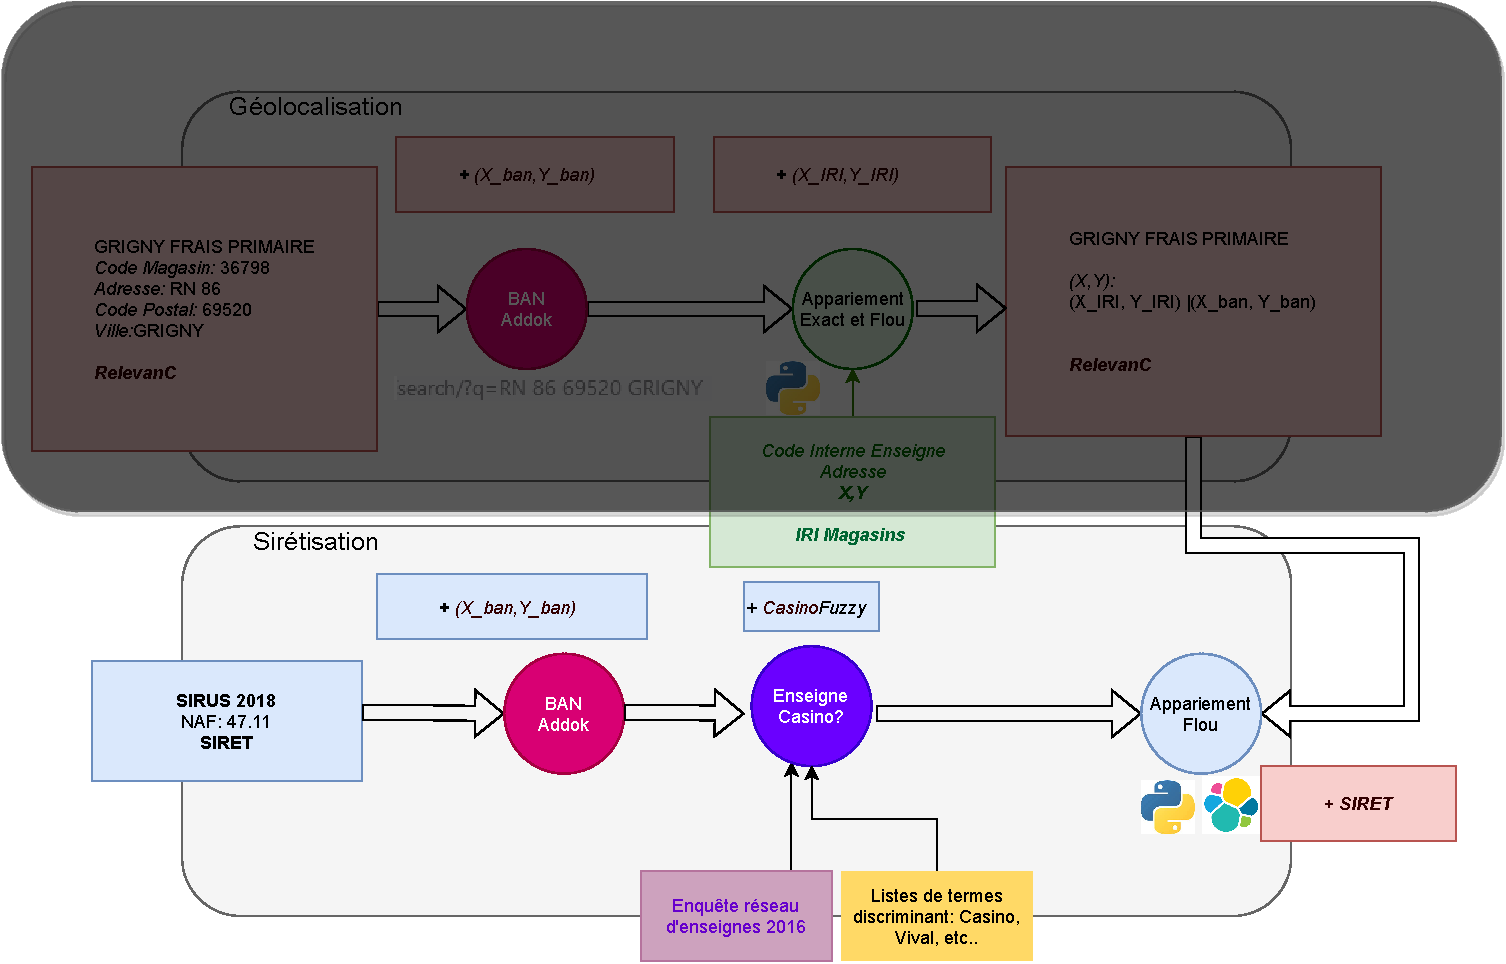
\includegraphics[width=0.98\paperwidth]{images/macro_siret.pdf}}
\end{frame}

\begin{frame}{Siretisation}
\begin{enumerate}
    \item Appariement Flou: à l'aide de la librarie python \textit{recordLinkages} ($\approx$ IRI)
    \item Complétée, pour les magasins au plus gros CA (e.g. Géant Casino) par des recherches "à la main" via Elastic
\end{enumerate}

Recherche d'un match dans
\begin{enumerate}
    \item SIRUS 47.11, suceptible d'appartenir à l'enseigne Casino
    \begin{itemize}
    \item (CP) \textit{Blocage:} Code Postal; \textit{Champ comparé et noté:} Nom du magasin, Libellé d'enseigne, Adresse Ban \textit{(string)}, X,Y \textit{(Point géographique)}, \textit{Embedding 3D Nom du magasin + Enseigne} \textit{(Numeric)}
    \end{itemize}
    \item SIRUS 47.11 
    \begin{itemize}
        \item (CP)
    \end{itemize}
    \item SIRUS 47.11 
    \begin{itemize}
        \item  (DEP) \textit{Blocage:} Département; \textit{Champ comparé et noté:} Nom du magasin, Libellé d'enseigne, Adresse, Ville \textit{(string)} et X,Y \textit{(Point géographique)} , \textit{Embedding 3D Nom du magasin + Enseigne} \textit{(Numeric)}
\end{itemize}
\end{enumerate}

\end{frame}

\begin{frame}{Exemples aléatoires}{1}
    \begin{tiny}
\begin{tabular}{lc}
\toprule
\rowcolor{LightCyan}
1 & PS ALLIGNY COSNE VIVAL\textbar 18 ROUTE DE BOUHY\textbar ALLIGNY COSNE \\ 
2 & NICE RAOUL BOSIO SPAR\textbar 2 BIS RUE RAOUL BOSIO\textbar NICE \\ 
\rowcolor{LightCyan}
3 & LP BASSENS LEADER PRICE\textbar 23 AV DE LA SOMME\textbar BASSENS \\ 
4 & PS DOMENE LE PETIT CASINO\textbar PLACE DE STALINGRAD\textbar DOMENE \\ 
\rowcolor{LightCyan}
5 & SEBASTOPOL FRANPRIX\textbar 12-14 RUE SANTEUIL\textbar PARIS \\ 
6 & SM CASINO ST PIERRE SUR DIVES SUPERMARCHE HYPER\textbar ROUTE DE LISIEUX\textbar ST PIERRE SUR DIVES \\ 
\rowcolor{LightCyan}
7 & POINT RETRAIT SM HARDRICOURT\textbar 60 RUE DU VEXIN\textbar HARDRICOURT \\ 
8 & ALYE FRANPRIX\textbar RUE HENRI SPAAK\textbar VERNOUILLET \\ 
\rowcolor{LightCyan}
9 & NEWFPMAG MONTROUGE FRANPRIX\textbar 37 RUE BARBES\textbar MONTROUGE \\ 
\bottomrule
\end{tabular}

\begin{tabular}{lc}
\toprule
\rowcolor{LightCyan}
1 & VIVAL AUX GOURMETS\textbar 18 ROUTE DE BOUHY 58200 ALLIGNY-COSNE \\ 
2 & SPAR NISACOL\textbar 2 BIS RUE RAOUL BOSIO 06300 NICE \\ 
\rowcolor{LightCyan}
3 & LEADER PRICE BASSENS\textbar AVENUE DE LA SOMME 33530 BASSENS \\ 
4 & DISTRIBUTION CASINO FRANCE LE PETIT DE DOMENE\textbar PLACE STALINGRAD 38420 DOMENE \\ 
\rowcolor{LightCyan}
5 & SEBASTOPOL DISTRIBUTION\textbar 14 RUE SANTEUIL 75005 PARIS \\ 
6 & DISTRIBUTION CASINO FRANCE\textbar RUE DE LISIEUX 14170 SAINT-PIERRE-EN-AUGE \\ 
\rowcolor{LightCyan}
7 & DISTRIBUTION CASINO FRANCE\textbar 60 RUE DU VEXIN 78250 HARDRICOURT \\ 
8 & NEWDNERA FRANPRIX\textbar RUE PAUL HENRI SPAACK 28500 VERNOUILLET \\ 
\rowcolor{LightCyan}
9 & FRANPRIX MONTROUGE MARKET\textbar 37 RUE BARBES 92120 MONTROUGE \\ 
\bottomrule
\end{tabular}


\end{tiny}
\end{frame}

\begin{frame}{Exemples aléatoires}{2}
    \begin{tiny}
\begin{tabular}{lc}
\toprule
\rowcolor{LightCyan}
1 & SM CASINO GOURDON SUPERMARCHE\textbar 86 86 AVENUE GAMBETTA\textbar 46300\textbar GOURDON \\ 
2 & MIRANDA COROMA FRANPRIX\textbar 1 ROND-POINT DES FETES\textbar 91210\textbar DRAVEIL \\ \rowcolor{LightCyan}
3 & RIE SEPR LYON\textbar SEPR RUE DU PROFESSEUR ROCHAIX\textbar 69003\textbar LYON \\ 
4 & VALLAURIS ANCIENS COMBATTANTS VIVAL\textbar 361 AV A COMB AFRIQUE NORD\textbar 06220\textbar VALLAURIS \\ 
\bottomrule
\end{tabular}

\begin{tabular}{lc}
\toprule
\rowcolor{LightCyan}
1 & SUPERMARCHE CASION DPR DISTRIBUTION\textbar 86 AVENUE GAMBETTA 46300 GOURDON \\ 
2 & COMPTOIR ROYAL MAROCAIN D ALIMENTATION\textbar 1 ROND POINT DES FETES 91210 DRAVEIL \\ 
\rowcolor{LightCyan}
3 & LPE ALIMENTATION\textbar RUE PROFESSEUR ROCHAIX 69003 LYON \\ 
4 & VIVAL SJ DISTRIB\textbar 361 AV A COMBATTANTS AFRIQUE NORD 06220 VALLAURIS \\ 
\bottomrule
\end{tabular}


\end{tiny}
\end{frame}
\begin{frame}{Exemples aléatoires}{3}
    \begin{tiny}
\begin{tabular}{lc}
\toprule
\rowcolor{LightCyan}
1 & LP ROINVILLE SOUS AUNEAU LEADER PRICE\textbar LA FOSSE FONDUE\textbar 28700\textbar ROINVILLE \\ 
2 & LP NEUILLY SUR MARNE LEADER PRICE\textbar 66/68 AV DU GENERAL DE GAULLE\textbar 93300\textbar NEUILLY SUR MARNE \\ 
\rowcolor{LightCyan}
3 & SM CASINO PARIS ST DIDIER SUPERMARCHE\textbar 16 RUE DES BELLES FEUILLES\textbar 75016\textbar PARIS \\ 
4 & LP ANGERS DBA LEADER PRICE\textbar DE LA CROIX BLANCHE\textbar 49000\textbar ANGERS \\ 
\bottomrule
\end{tabular}

\begin{tabular}{lc}
\toprule
\rowcolor{LightCyan}
1 & LEADER PRICE ROINVILLE\textbar FOSSE FONDUE 28700 ROINVILLE \\ 
2 & NEUILLY DISTRIBUTION\textbar 68 AVENUE DU GENERAL DE GAULLE 93330 NEUILLY-SUR-MARNE \\ 
\rowcolor{LightCyan}
3 & DISTRIBUTION CASINO FRANCE\textbar 16 RUE DES BELLES FEUILLES 75016 PARIS \\ 
4 & LEADER PRICE BELRIV ANGERS\textbar RUE DE LA CROIX BLANCHE 49100 ANGERS \\ 
\bottomrule
\end{tabular}


\end{tiny}
\end{frame}
\section{Conclusion}\label{sec: conclusion}


\end{document}
